\section{结果与讨论}

在这部分中,我们评估了所提出的噪声检测分类方法的性能,用于评测的ECG信号包含了不同形态的PQRST波,其中包括了BW噪声、ABC噪声,PLI噪声和肌电干扰噪声等多种噪声。在本研究中,第一个决策阶段首先检测了低频噪声(BW噪声和ABC噪声)和高频噪声(PLI噪声和肌电干扰噪声)是否存在。在第二个决策阶段,低频组分和高频组分被归类为BW噪声、ABC噪声,PLI噪声和肌电干扰这几类。该ECG噪声检测归类方法的简易流程图见图6。
\begin{figure}[htbp]
\label{figNo.6}
\centering
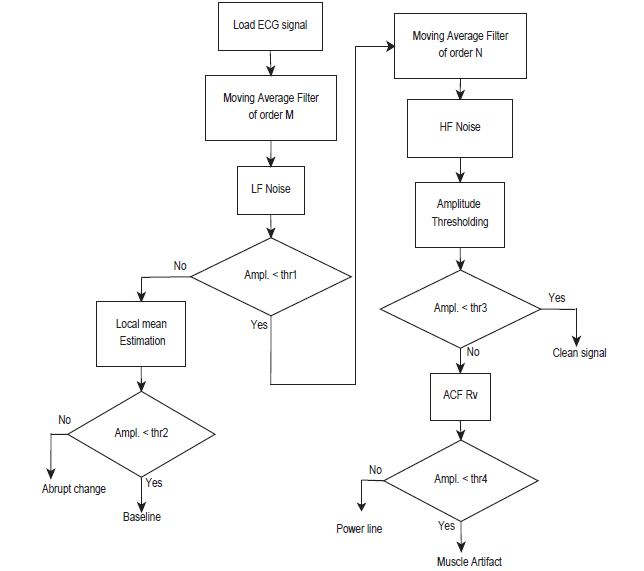
\includegraphics[width=0.7\columnwidth]{fig6.jpg}
\caption{本文中ECG噪声检测和分类方法的简易流程图
}
\end{figure}

对于性能评估方法,使用MIT-BIH心律失常数据库(MIT-BIH Arrhythmia Database, mitadb)中的ECG记录构建了大规模ECG测试信号数据库。这些ECG信号的采样率为360Hz,分辨率为11-bit。ECG测试信号数据库共含有150条ECG信号记录。每个ECG测试信号的记录时常为10s。大规模ECG测试信号数据库中的信号加入了各种不同噪声级别的噪声。这些合成的噪声通过文献21中的软件包生成。分类结果与真实数据的对比见表\ref{tab2}。

性能测试中,灵敏度Se,效率+P和精确度三种测试评分计算如下:
\begin{equation}
  Se=\frac{\mathrm{TP}}{\mathrm{TP+FN}} \times 100
  \label{equ9}
\end{equation}

\begin{equation}
  \mathrm{+P}=\frac{\mathrm{TP}}{\mathrm{TP+FP}} \times 100
  \label{equ10}
\end{equation}

\begin{equation}
  Accuracy=\frac{\mathrm{TP}}{\mathrm{TP+FN+FP}} \times 100
  \label{equ11}
\end{equation}
其中TP(True Positive)表示算法正确分类了测试片段,FP(False Positive)表示算法将测试片段错误地分为了某类噪声,FN(False Negative)表示测试片段所含的噪声类型分类错误。表\ref{tab3}总结了本文所提出方法的测试评分结果。对于大部分类型的噪声(除了ABC、PLI混合噪声以及ABC、MA混合噪声),该方法的分类准确度达到了85\%以上。表\ref{tab4}给出了本分类方法的混淆矩阵。
\begin{table}[htbp]
\scriptsize
  \centering
  \caption{噪声检测分类算法结果与真实结果比较 % 表头
  \label{tab2}}
\begin{tabular}{|c|c|c|c|c|c|c|c|c|c|}
\hline 
波形记录 & \multicolumn{9}{c|}{真实情况} \\ 
\hline 
~~ & 非带噪信号 & BW & ABC & MN & PL & BW+PL & BW+MN & ABC+PL & ABC+MN \\ 
\hline 
100 & 9 & 66 & 21 & 5 & 23 & 1 & 25 & 0 & 0 \\ 
\hline 
101 & 2 & 74 & 9 & 0 & 4 & 14 & 43 & 2 & 2 \\ 
\hline 
102 & 4 & 68 & 23 & 0 & 26 & 0 & 29 & 0 & 0 \\ 
\hline 
103 & 6 & 74 & 16 & 15 & 23 & 1 & 15 & 0 & 0 \\ 
\hline 
104 & 3 & 41 & 7 & 5 & 5 & 10 & 73 & 0 & 6 \\ 
\hline 
105 & 6 & 66 & 18 & 0 & 24 & 2 & 34 & 0 & 0 \\ 
\hline 
106 & 19 & 55 & 13 & 15 & 18 & 6 & 21 & 0 & 3 \\ 
\hline 
107 & 18 & 111 & 8 & 0 & 5 & 8 & 0 & 0 & 0 \\ 
\hline 
108 & 4 & 23 & 18 & 1 & 4 & 11 & 86 & 0 & 3 \\ 
\hline 
109 & 11 & 72 & 19 & 16 & 17 & 1 & 14 & 0 & 0 \\ 
\hline 
111 & 4 & 77 & 7 & 6 & 7 & 15 & 33 & 0 & 1 \\ 
\hline 
总数 & 86 & 727 & 159 & 63 & 156 & 69 & 373 & 2 & 15 \\ 
\hline 
波形记录 & \multicolumn{9}{c|}{算法分类结果} \\ 
\hline 
~~ & 非带噪信号 & BW & ABC & MN & PL & BW+PL & BW+MN & ABC+PL & ABC+MN \\ 
\hline 
100 & 8 & 62 & 25 & 6 & 20 & 4 & 24 & 1 & 0 \\ 
\hline 
101 & 3 & 85 & 15 & 0 & 2 & 10 & 34 & 0 & 1 \\ 
\hline 
102 & 8 & 70 & 25 & 3 & 20 & 5 & 15 & 1 & 1 \\ 
\hline 
103 & 4 & 71 & 20 & 21 & 21 & 5 & 8 & 0 & 0 \\ 
\hline 
104 & 2 & 34 & 5 & 8 & 3 & 8 & 81 & 0 & 9 \\ 
\hline 
105 & 9 & 61 & 15 & 1 & 28 & 3 & 32 & 0 & 1 \\ 
\hline 
106 & 17 & 51 & 15 & 15 & 20 & 8 & 23 & 0 & 1 \\ 
\hline 
107 & 20 & 108 & 11 & 4 & 4 & 3 & 0 & 0 & 0 \\ 
\hline 
108 & 1 & 15 & 14 & 9 & 3 & 10 & 91 & 1 & 6 \\ 
\hline 
109 & 14 & 75 & 17 & 14 & 14 & 1 & 15 & 0 & 0 \\ 
\hline 
111 & 2 & 82 & 10 & 8 & 3 & 11 & 34 & 0 & 0 \\ 
\hline 
总数 & 88 & 714 & 172 & 89 & 138 & 68 & 357 & 3 & 21 \\ 
\hline 
\end{tabular} 
\end{table}
基于表\ref{tab3}和表\ref{tab4}的结果可以认为,我们提出的方法适用于大多数常见噪声的检测,其中包括BW、PLI、ABC、MA噪声,以及BW/PLI混合噪声、BW/MA混合噪声。

\begin{table}[htp]
\scriptsize
\centering
\caption{本文中分类方法的混淆矩阵 % 表头
\label{tab4}}
\begin{tabular}{|c|c|c|c|c|c|c|c|c|c|}
\hline 
~~ & 非带噪信号 & BW & ABC & MN & PL & BW+PL & BW+MN & ABC+PL & ABC+MN \\ 
\hline 
非带噪信号 & 86 & 2 & - & - & - & - & - & - & - \\ 
\hline 
BW & 3 & 714 & - & 2 & - & - & 8 & - & - \\ 
\hline 
ABC & - & 3 & 159 & - & - & - & 6 & - & 4 \\ 
\hline 
MN & - & - & 4 & 63 & 2 & - & 14 & - & 6 \\ 
\hline 
PL & - & - & - & 7 & 138 & 9 & - & 2 & - \\ 
\hline 
BW+PL & - & - & - & - & - & 68 & 1 & - & - \\ 
\hline 
BW+MN & - & - & - & 8 & - & - & 357 & - & 8 \\ 
\hline 
ABC+PL & - & - & - & 1 & - & - & - & 2 & - \\ 
\hline 
ABC+MN & - & - & - & - & - & - & 5 & 1 & 15 \\ 
\hline 
\end{tabular} 
\end{table}
\begin{table}[htp]
\small
\centering
\caption{本文方法的分类结果 % 表头
\label{tab3}}
\begin{tabular}{|r|c|c|c|c|c|c|c|}
\hline 
信号类型 & 信号片段数量 & TP & FP & FN & Se(\%) & +P(\%) & 准确度(\%) \\ 
\hline 
非带噪信号 & 86 & 86 & 2 & - & 100 & 97.72 & 97.72 \\ 
\hline 
BW & 727 & 714 & - & 13 & 98.21 & 100 & 98.21 \\ 
\hline 
ABC & 159 & 159 & 13 & - & 100 & 92.44 & 92.44 \\ 
\hline 
MN & 63 & 63 & 26 & - & 100 & 92.44 & 92.44 \\ 
\hline 
PL & 156 & 138 & - & 18 & 88.46 & 100 & 88.46 \\ 
\hline 
BW+PL & 69 & 68 & - & 1 & 98.55 & 100 & 98.55 \\ 
\hline 
BW+MN & 373 & 357 & - & 16 & 95.71 & 100 & 95.71 \\ 
\hline 
ABC+PL & 2 & 2 & 1 & - & 100 & 66.66 & 66.66 \\ 
\hline 
ABC+MN & 15 & 15 & 6 & - & 100 & 71.42 & 71.42 \\ 
\hline 
总数 & 1650 & 1602 & 48 & 48 & 97.88 & 91.18 & 89.06 \\ 
\hline 
\end{tabular}   
\end{table}

之后,本研究将着眼于提高本文方法在检测、分类其他混合类型噪声上的性能。相较于其他现行噪声检测分类方法中的信号分离技术、特征提取技术和监督分类器,本文方法的滤波、特征提取和分类技术十分简单。而可穿戴心脏疾病监护设备由于其电量少、存储空间小、计算速率低的特点,正需要一种低复杂度的信号质量评测方法。基于我们的分类结果,我们认为本文提出的方法对于评估Holter和动态ECG信号的质量具有很高的适用性。
